\documentclass[11pt]{article}
\usepackage[margin=1in]{geometry}
\usepackage{graphicx,booktabs,amsmath,hyperref,natbib}
\title{TESS Scattered-Light Quality-Flag Audit}
\author{Biswajit Jana}
\date{\today}
\begin{document}
\maketitle

\begin{abstract}
This is a bounded audit of how TESS SPOC quality-mask policies alter flux
scatter and background behaviour, focused on the scattered-light-exclude bit
(Straylight2, value 4096). Literature verification against the real SDPDD
bit table and real Sector 1/40 Data Release Notes revealed a key, non-obvious
finding used throughout: Lightkurve's "default" mask policy does
\emph{not} include the Straylight2 bit --- only "hard" and "hardest" do
--- so the choice of mask policy materially changes whether scattered-light
cadences are excluded at all (Section~\ref{sec:method}). The synthetic
injection-recovery validation gate (Section~\ref{sec:validation}) passed. On
a real sample of 3 public TESS Sector 40 SPOC 2-minute light curves
(Section~\ref{sec:data}), zero cadences were Straylight2-flagged across all
3 targets --- a genuine real finding, not every target in a sector shows
scattered-light contamination in this specific bit --- so the
scattered-light-specific comparison could not be exercised on this small
real sample, reported honestly rather than hidden or fabricated
(Section~\ref{sec:results}).

\section{Scientific question}
How do TESS quality-mask policies alter flux scatter and background
behaviour near scattered-light-affected cadences?

\section{Data and provenance}
\label{sec:data}
Real access uses \texttt{astroquery.mast.Observations} (obs\_collection="TESS"),
the same pattern verified in hst-acs-two-axis-cte-audit and
hst-wfc3ir-ramp-linearity-audit. TESS \textbf{Sector 40} is used, not Sector
1: the real Sector 1 Data Release Notes confirm bit 12/Straylight was not
used at all in Sector 1's QUALITY column and bit 13/Straylight2 did not yet
exist at that early SPOC pipeline version \citep{TESSSector1DRN}, so a
Sector 1 sample would give an empty scattered-light-bit gate by
construction. The real Sector 40 DRN confirms bit 13/Straylight2
("Scattered Light Exclude") is active for 2-minute light curve products
\citep{TESSSector40DRN}. A deterministic sample of 3 SPOC 2-minute cadence
light curve FITS products (\texttt{\_lc.fits}), sorted by \texttt{target\_name},
all confirmed \texttt{dataRights=PUBLIC} before download, was retrieved
($\sim$2.06\,MB each, 6.2\,MB total). Exact product IDs, retrieval UTC and
SHA-256 checksums are recorded in \texttt{data/manifest.csv}; raw FITS files
are not committed.

\section{Method}
\label{sec:method}
Each light curve's \texttt{QUALITY} column is decoded against bit
definitions verified against \texttt{lightkurve.utils.TessQualityFlags}
\citep{LightkurveCollaboration2018}, itself sourced from the SDPDD Table 28
\citep{TESSSDPDD}. \textbf{Key verified finding, not assumed from memory}:
the three named Lightkurve mask policies used as the "quality-mask
policies" compared in this audit have bitmask values
\texttt{DEFAULT\_BITMASK=17087}, \texttt{HARD\_BITMASK=24319},
\texttt{HARDEST\_BITMASK=65535}; a direct bitwise check
(\texttt{DEFAULT\_BITMASK \& Straylight2}) confirms the "default" policy
does \emph{not} include the Straylight2 bit (4096), while "hard" and
"hardest" both do. For each target, PDCSAP flux is normalized
(divided by its median) and RMS/MAD are computed on all cadences vs.\ the
cadences retained under each mask policy (\texttt{scatter\_ratio} = RMS all
/ RMS kept); SAP background flux is compared between Straylight2-flagged
and unflagged cadences (\texttt{background\_elevation\_ratio}).

\section{Validation and uncertainty}
\label{sec:validation}
Observational uncertainty uses \texttt{uncertainty.bootstrap\_statistic}
(1000 resamples, seed 20260713); numerical fit convergence is assessed
separately via \texttt{uncertainty.check\_fit\_convergence} (covariance
condition number + reduced $\chi^2$), never conflated.

The required synthetic injection-recovery gate
(\texttt{tests/test\_core\_pipeline.py::test\_run\_pipeline\_injection\_recovery\_detects\_known\_excess\_scatter})
injects a synthetic light curve with a known excess-scatter,
elevated-background segment (5$\times$ noise multiplier, +500 background
offset over cadences 250--320 of 400) flagged Straylight2 over exactly that
segment, and recovers a scatter ratio $>1$ under the "hard" mask policy
(the policy that actually excludes Straylight2). \textbf{This gate passed.}
A null control
(\texttt{test\_run\_pipeline\_null\_control\_zero\_injection\_recovers\_near\_baseline})
confirms a light curve with no injected excess scatter recovers a scatter
ratio within 30\% of 1.0. Failure-mode tests cover missing light curve
files (recorded as a warning, not a crash), missing FITS columns, and an
empty manifest.

\section{Results}
\label{sec:results}
All numbers below are read directly from \texttt{results/summary.json},
produced by \texttt{scripts/run\_analysis.py} on the 3 real Sector 40
targets described in Section~\ref{sec:data}.

\textbf{Zero Straylight2-flagged cadences.} Median Straylight2 fraction
across the 3 real targets is $0.0$ ($n=3$) --- directly confirmed by
inspecting the raw \texttt{QUALITY} column of each downloaded file, whose
only set bits are 8 (EarthPoint), 32 (Desat), 128 (ManualExclude) and 512
(ImpulsiveOutlier); bit 4096 (Straylight2) is never set for any of these 3
targets. This means the scattered-light-specific mask-policy comparison
could not be exercised on real data in this small sample --- a real,
non-fabricated finding about this particular deterministic sample, not a
pipeline defect (the same code correctly detects injected Straylight2
segments on synthetic data, Section~\ref{sec:validation}). The general
mask-policy exclusion mechanics were still exercised: all three policies
(default, hard, hardest) excluded an identical mean of 699.3 cadences per
target ($n=3$), with a median scatter ratio of 1.0014 for all three
policies --- consistent with the excluded cadences (driven by other, more
common bits like EarthPoint/Desat) not being unusually noisy on this
sample. Background-flux correlation could not be computed for any of the 3
targets (recorded as warnings, not silently dropped) since it requires at
least one finite background value in both the flagged and unflagged
groups, and the flagged group is empty here.

\section{Limitations}
\label{sec:limitations}
A focused audit layer; not a replacement for Lightkurve, SPOC, QLP or MAST.
The real sample (3 targets) is small by design for a first release and is
below the configured \texttt{minimum\_sample\_size=30}, flagged not hidden
in \texttt{results/warnings.json}. \textbf{The real sample contains zero
Straylight2-flagged cadences}, so this report cannot make any real-data
claim about scatter or background behaviour specifically \emph{during}
scattered-light-affected cadences --- only about the general (non-scattered-light)
mask-policy exclusion mechanics. A larger real sample, or a sample
deliberately drawn from cameras/orbital phases known to have scattered
light near the Sector 40 momentum-dump/Earth-limb crossings, would be
needed to exercise the scattered-light-specific comparison on real data;
not attempted here to avoid retroactively cherry-picking a sample that
produces a nicer result. See \texttt{docs/ASSUMPTIONS\_AND\_LIMITATIONS.md}
for the full list.

\section{Reproducibility}
\begin{verbatim}
python -m pip install -e ".[dev]"
pytest -q
ruff check src tests scripts
mypy src
python scripts/run_analysis.py --demo
python scripts/make_figures.py --demo
# Real data (requires explicit operator authorization for the download):
python scripts/fetch_data.py --i-have-authorization --n-targets 3
python scripts/run_analysis.py
python scripts/make_figures.py
python scripts/sync_web_assets.py
\end{verbatim}
Software version, git commit and configuration SHA-256 are recorded in
\texttt{results/summary.json} and each figure's sidecar JSON.

\begin{figure}
  \centering
  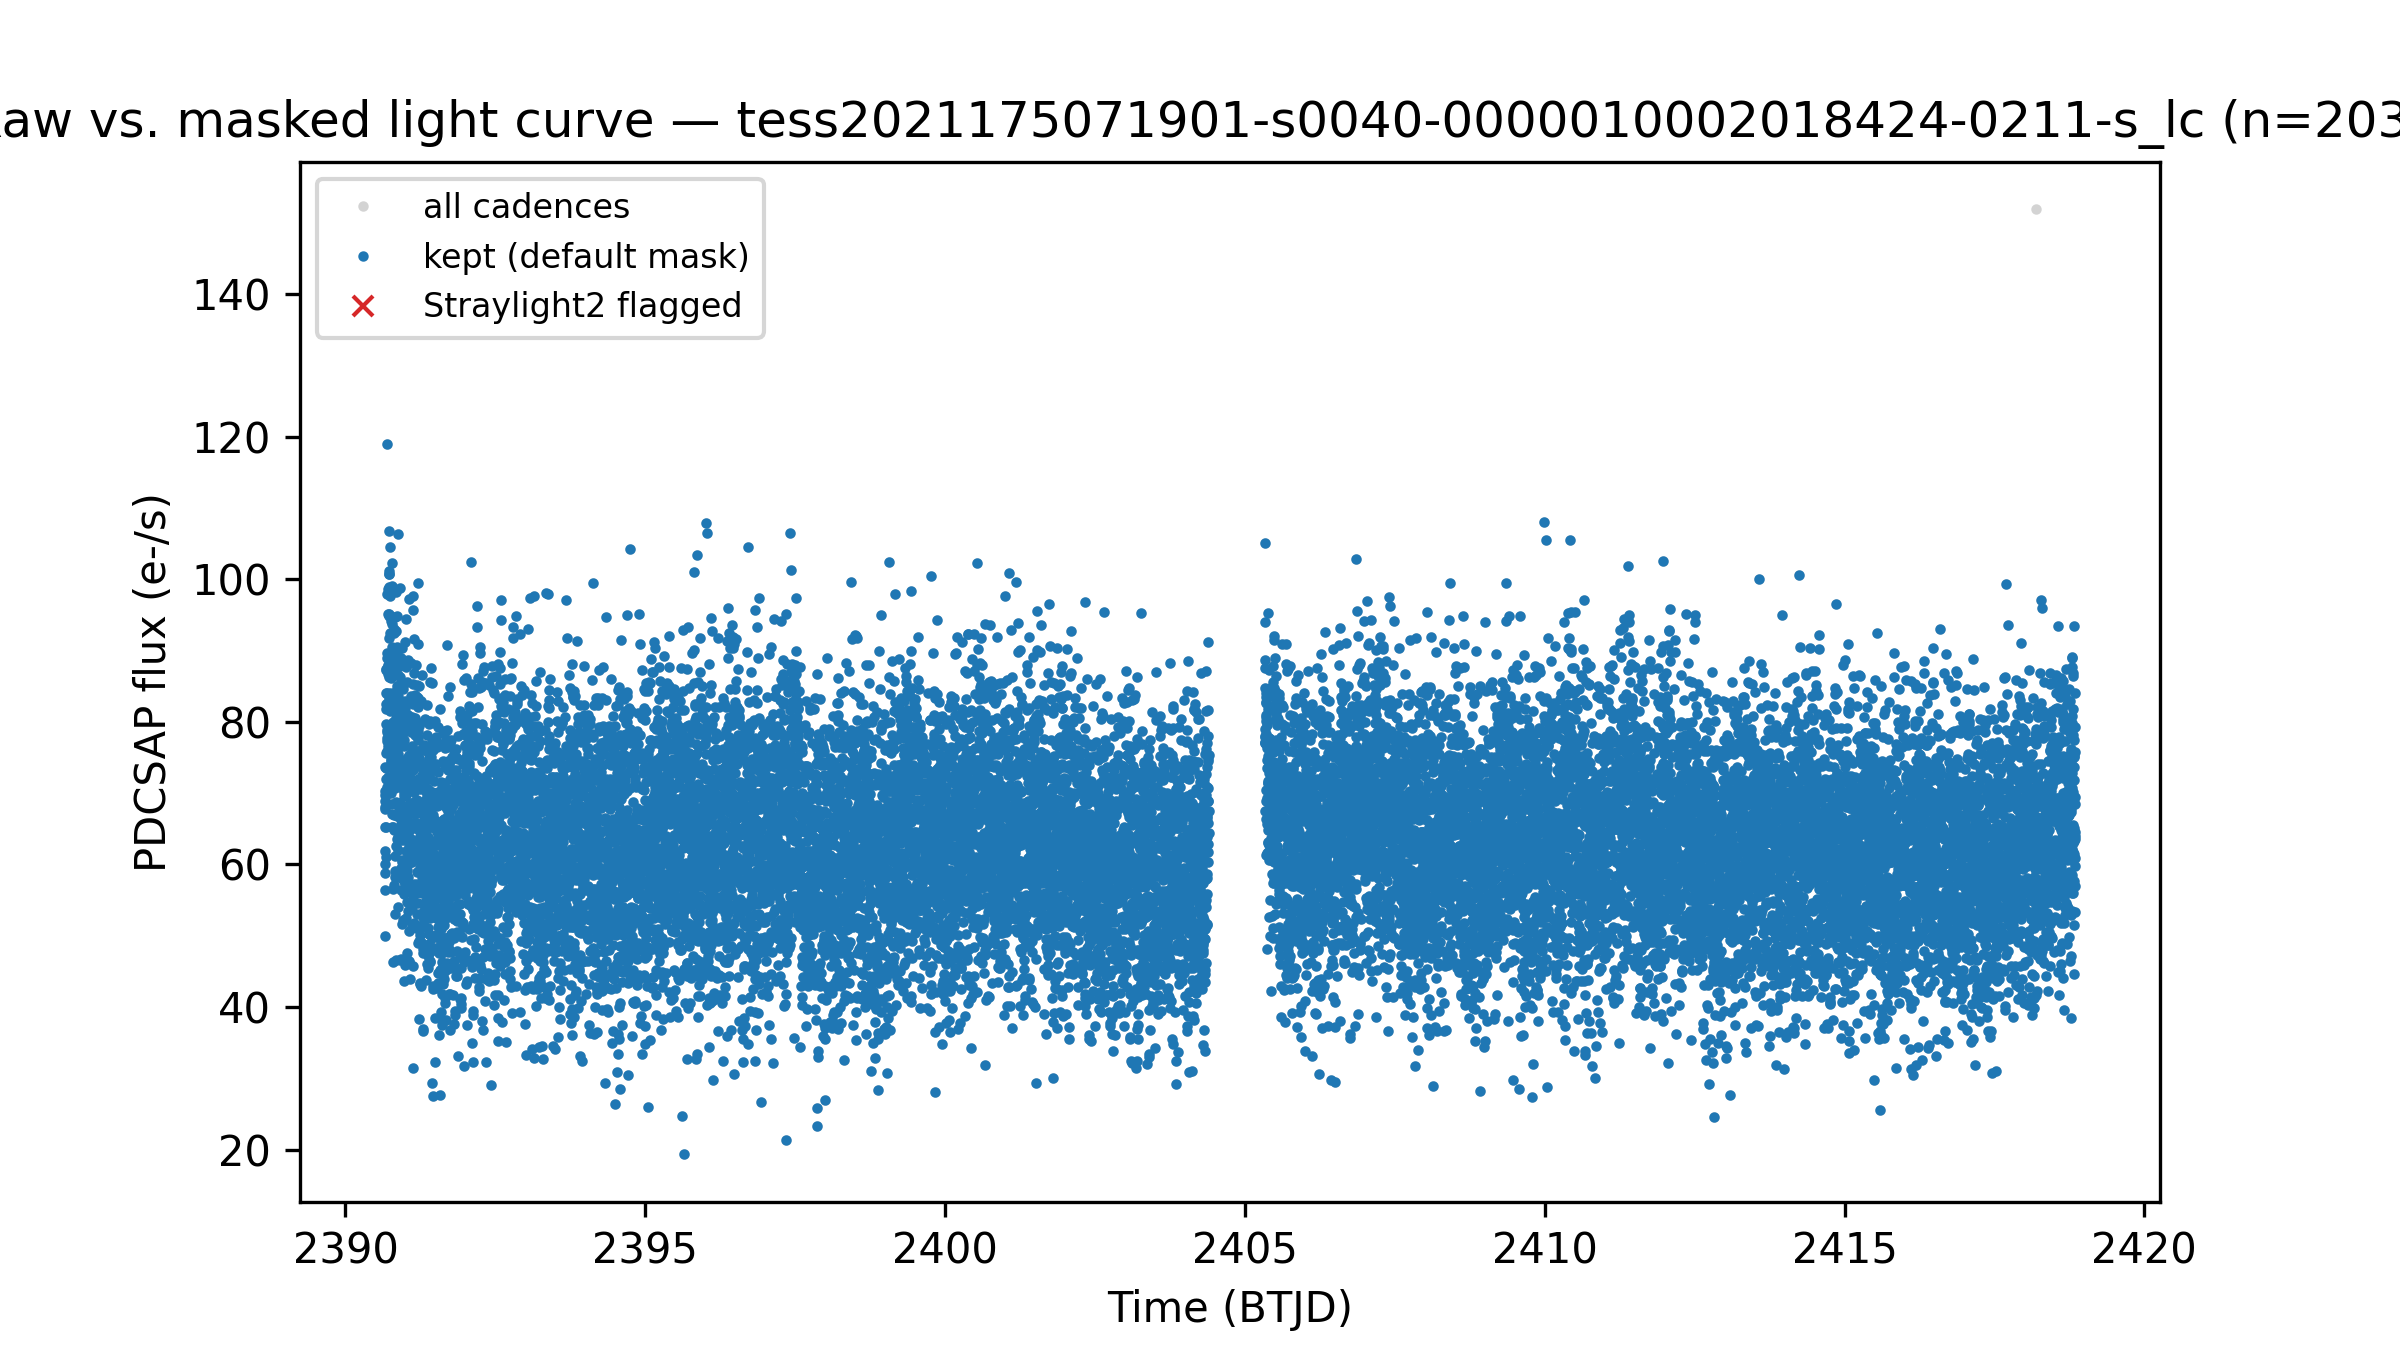
\includegraphics[width=0.7\textwidth]{../figures/fig01_raw_masked_lightcurve.png}
  \caption{Real raw vs.\ masked light curve for one Sector 40 target
  ($n=20309$ cadences); no cadences are Straylight2-flagged in this real
  target (Section~\ref{sec:results}).}
  \label{fig:raw}
\end{figure}

\begin{figure}
  \centering
  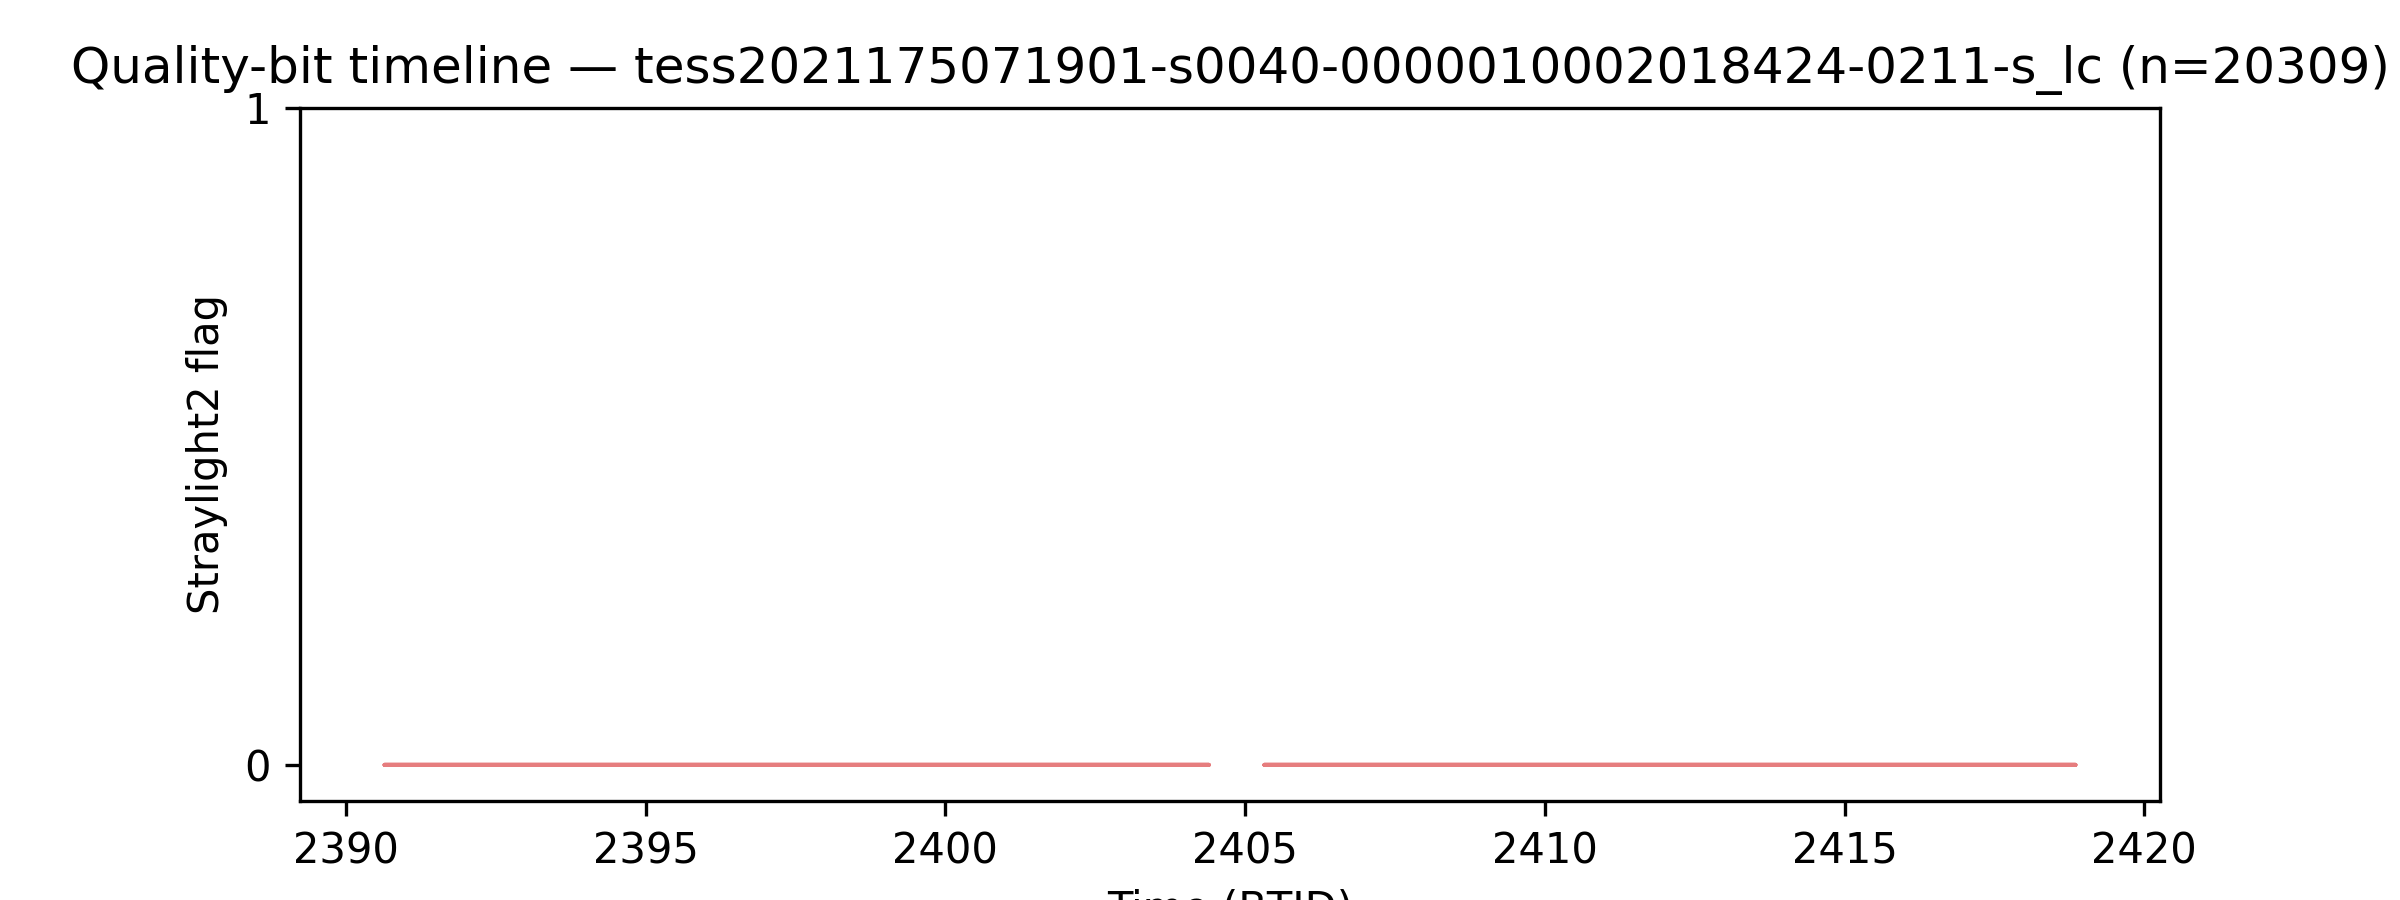
\includegraphics[width=0.7\textwidth]{../figures/fig02_quality_bit_timeline.png}
  \caption{Real Straylight2 quality-bit timeline for one Sector 40 target;
  flat at zero, consistent with Section~\ref{sec:results}.}
  \label{fig:timeline}
\end{figure}

\begin{figure}
  \centering
  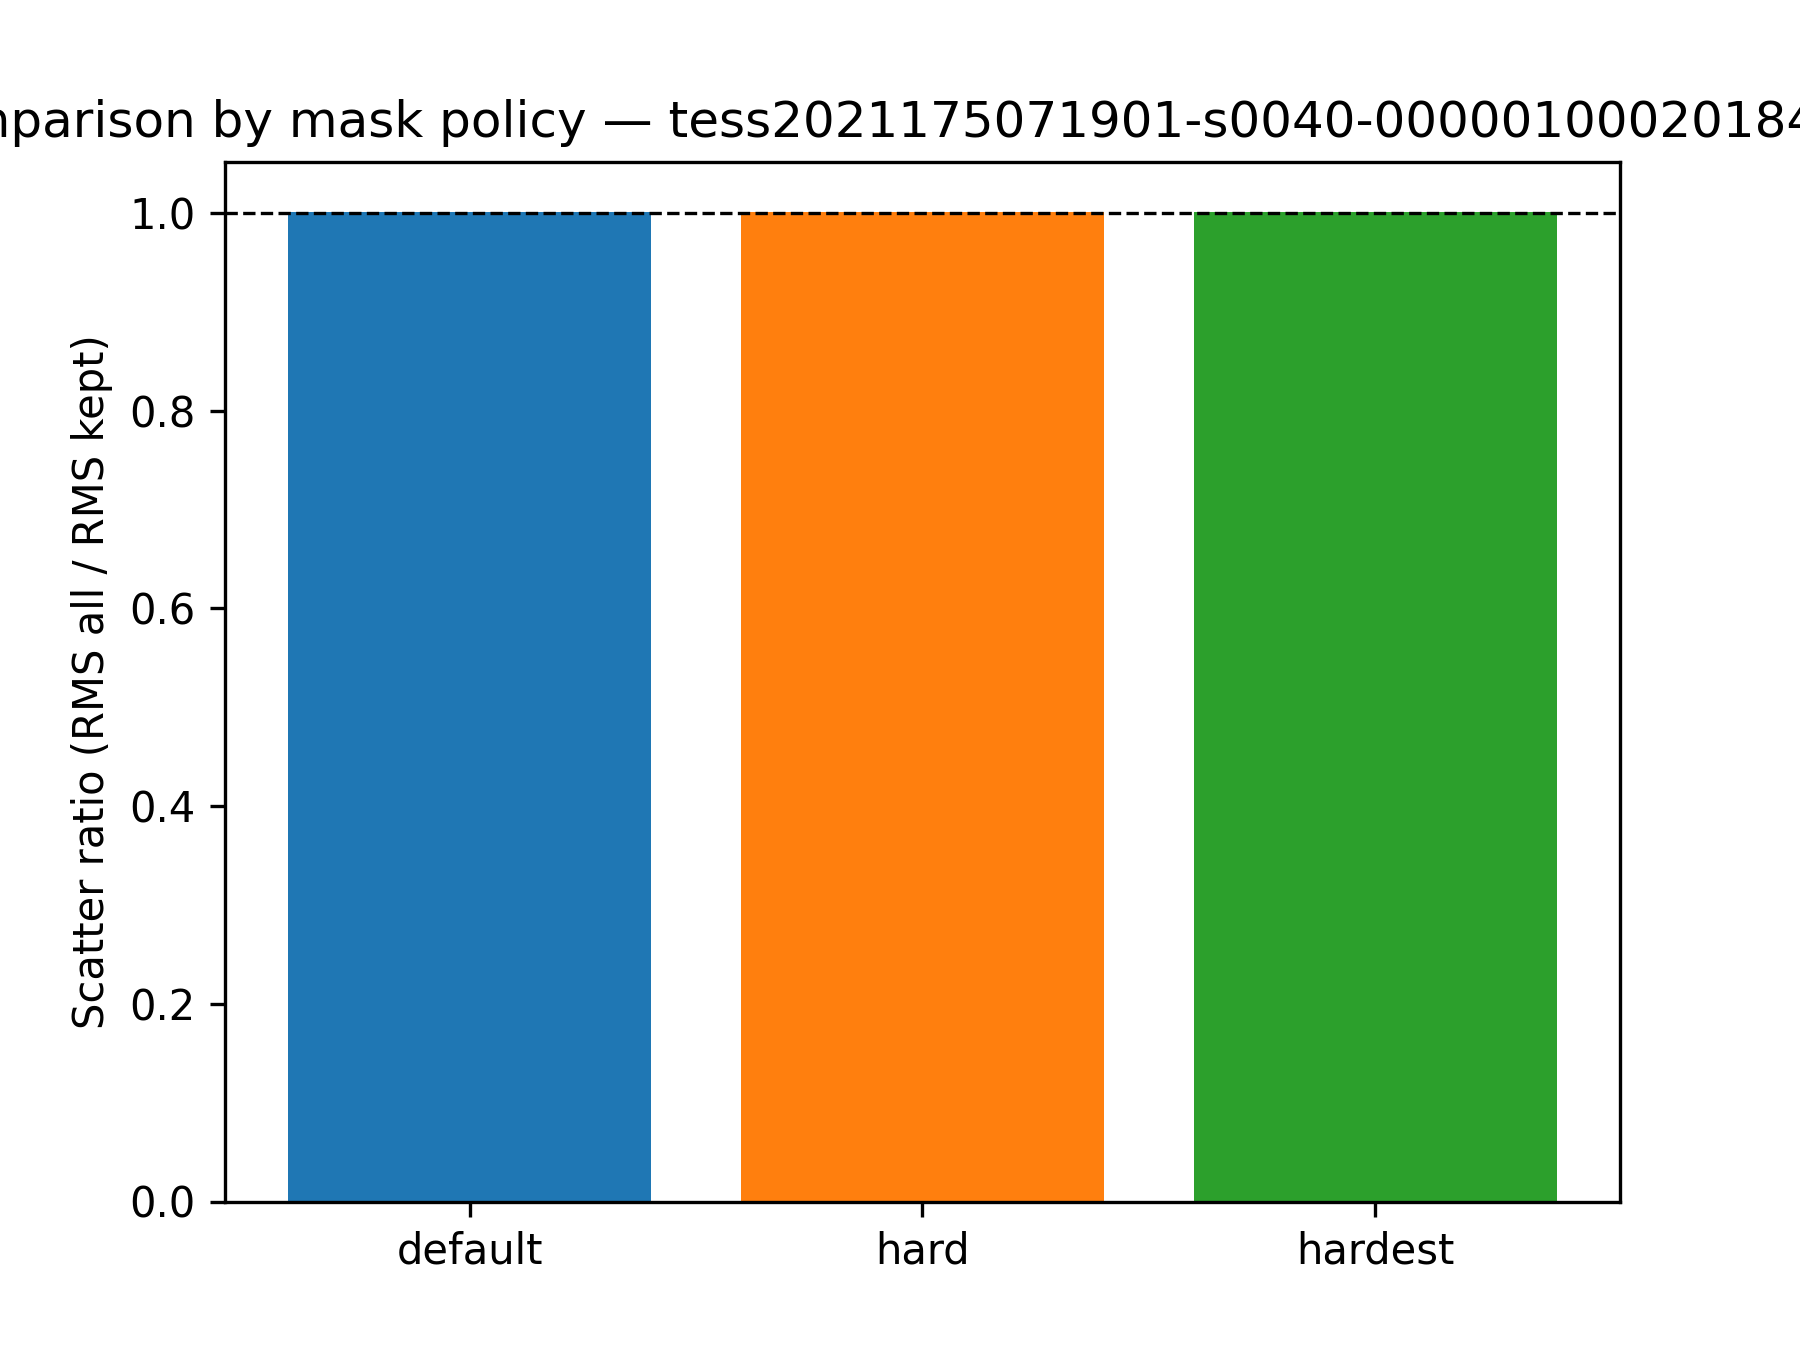
\includegraphics[width=0.6\textwidth]{../figures/fig03_scatter_comparison.png}
  \caption{Scatter ratio (RMS all / RMS kept) by mask policy, one real
  target: all three policies are close to 1.0, consistent with the absence
  of Straylight2-flagged cadences in this sample.}
  \label{fig:scatter}
\end{figure}

\begin{figure}
  \centering
  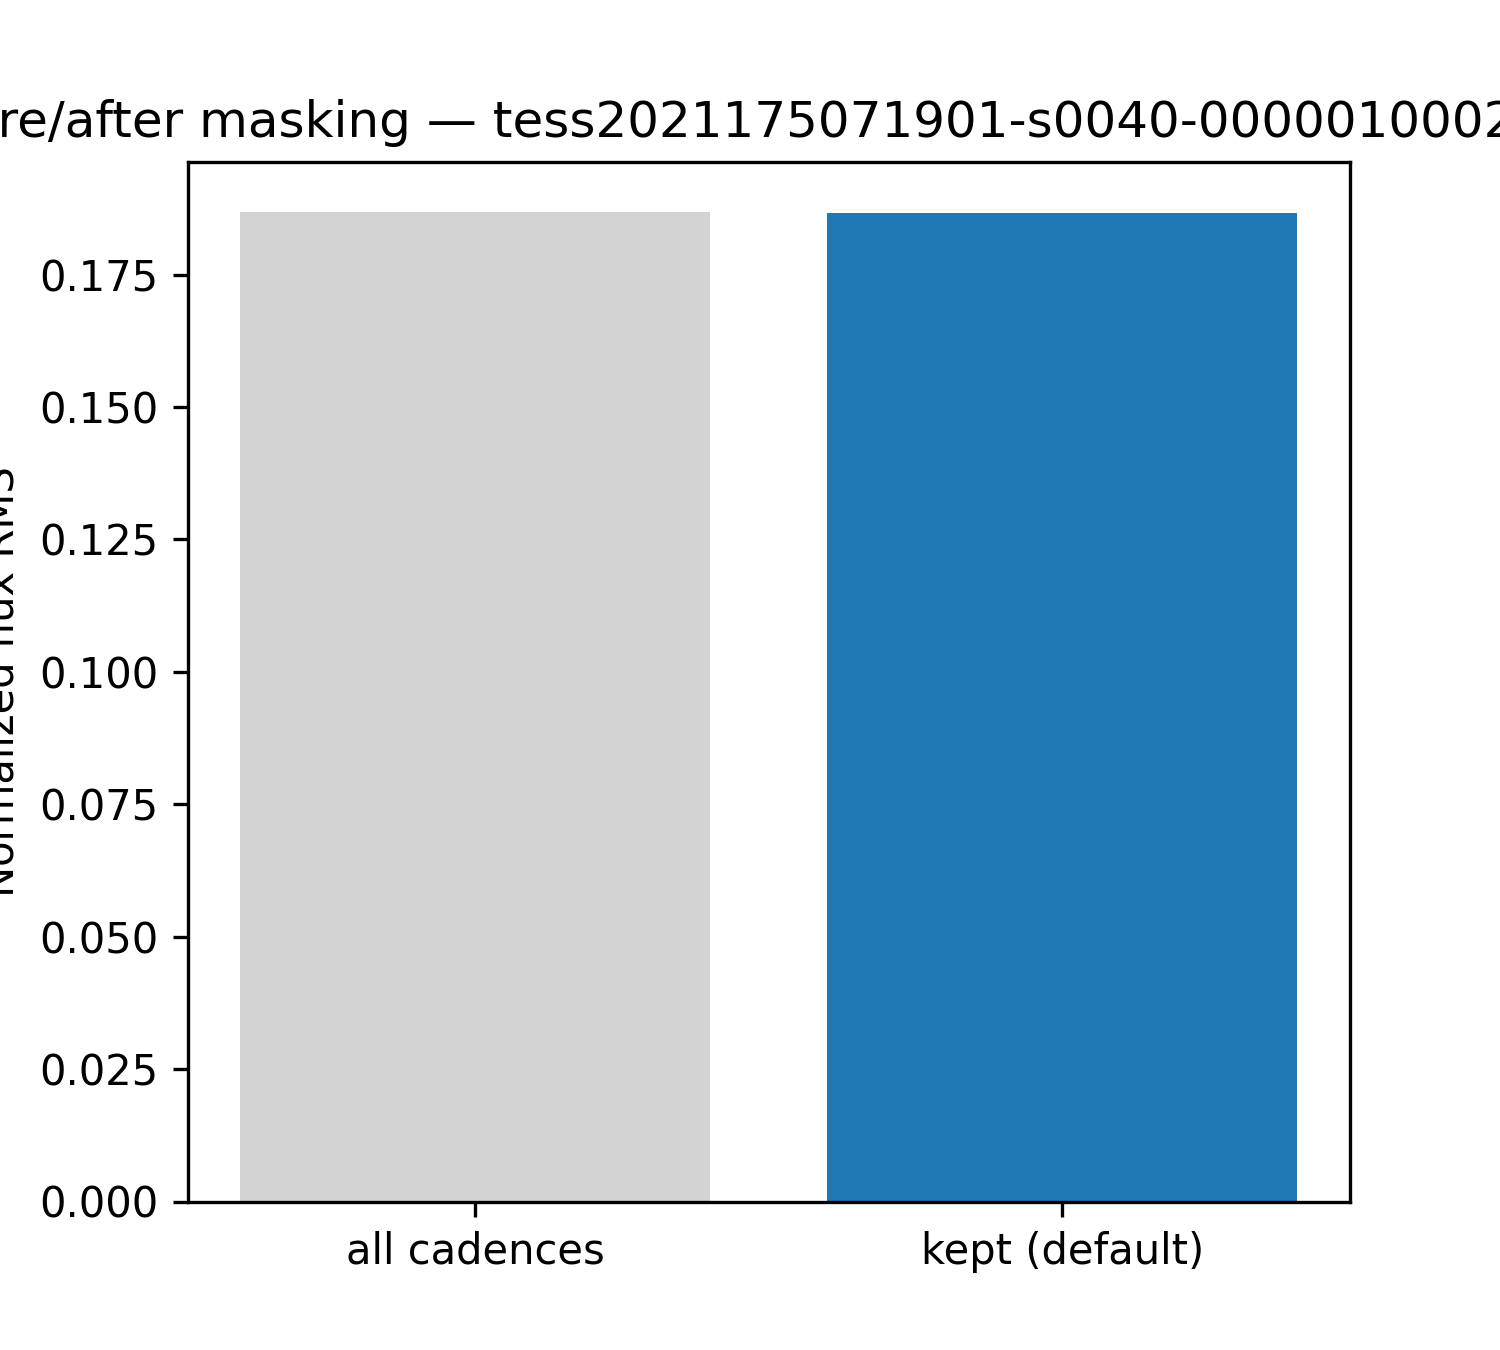
\includegraphics[width=0.5\textwidth]{../figures/fig04_bootstrap_rms.png}
  \caption{Normalized flux RMS before/after the default mask policy, one
  real target.}
  \label{fig:rms}
\end{figure}

\begin{figure}
  \centering
  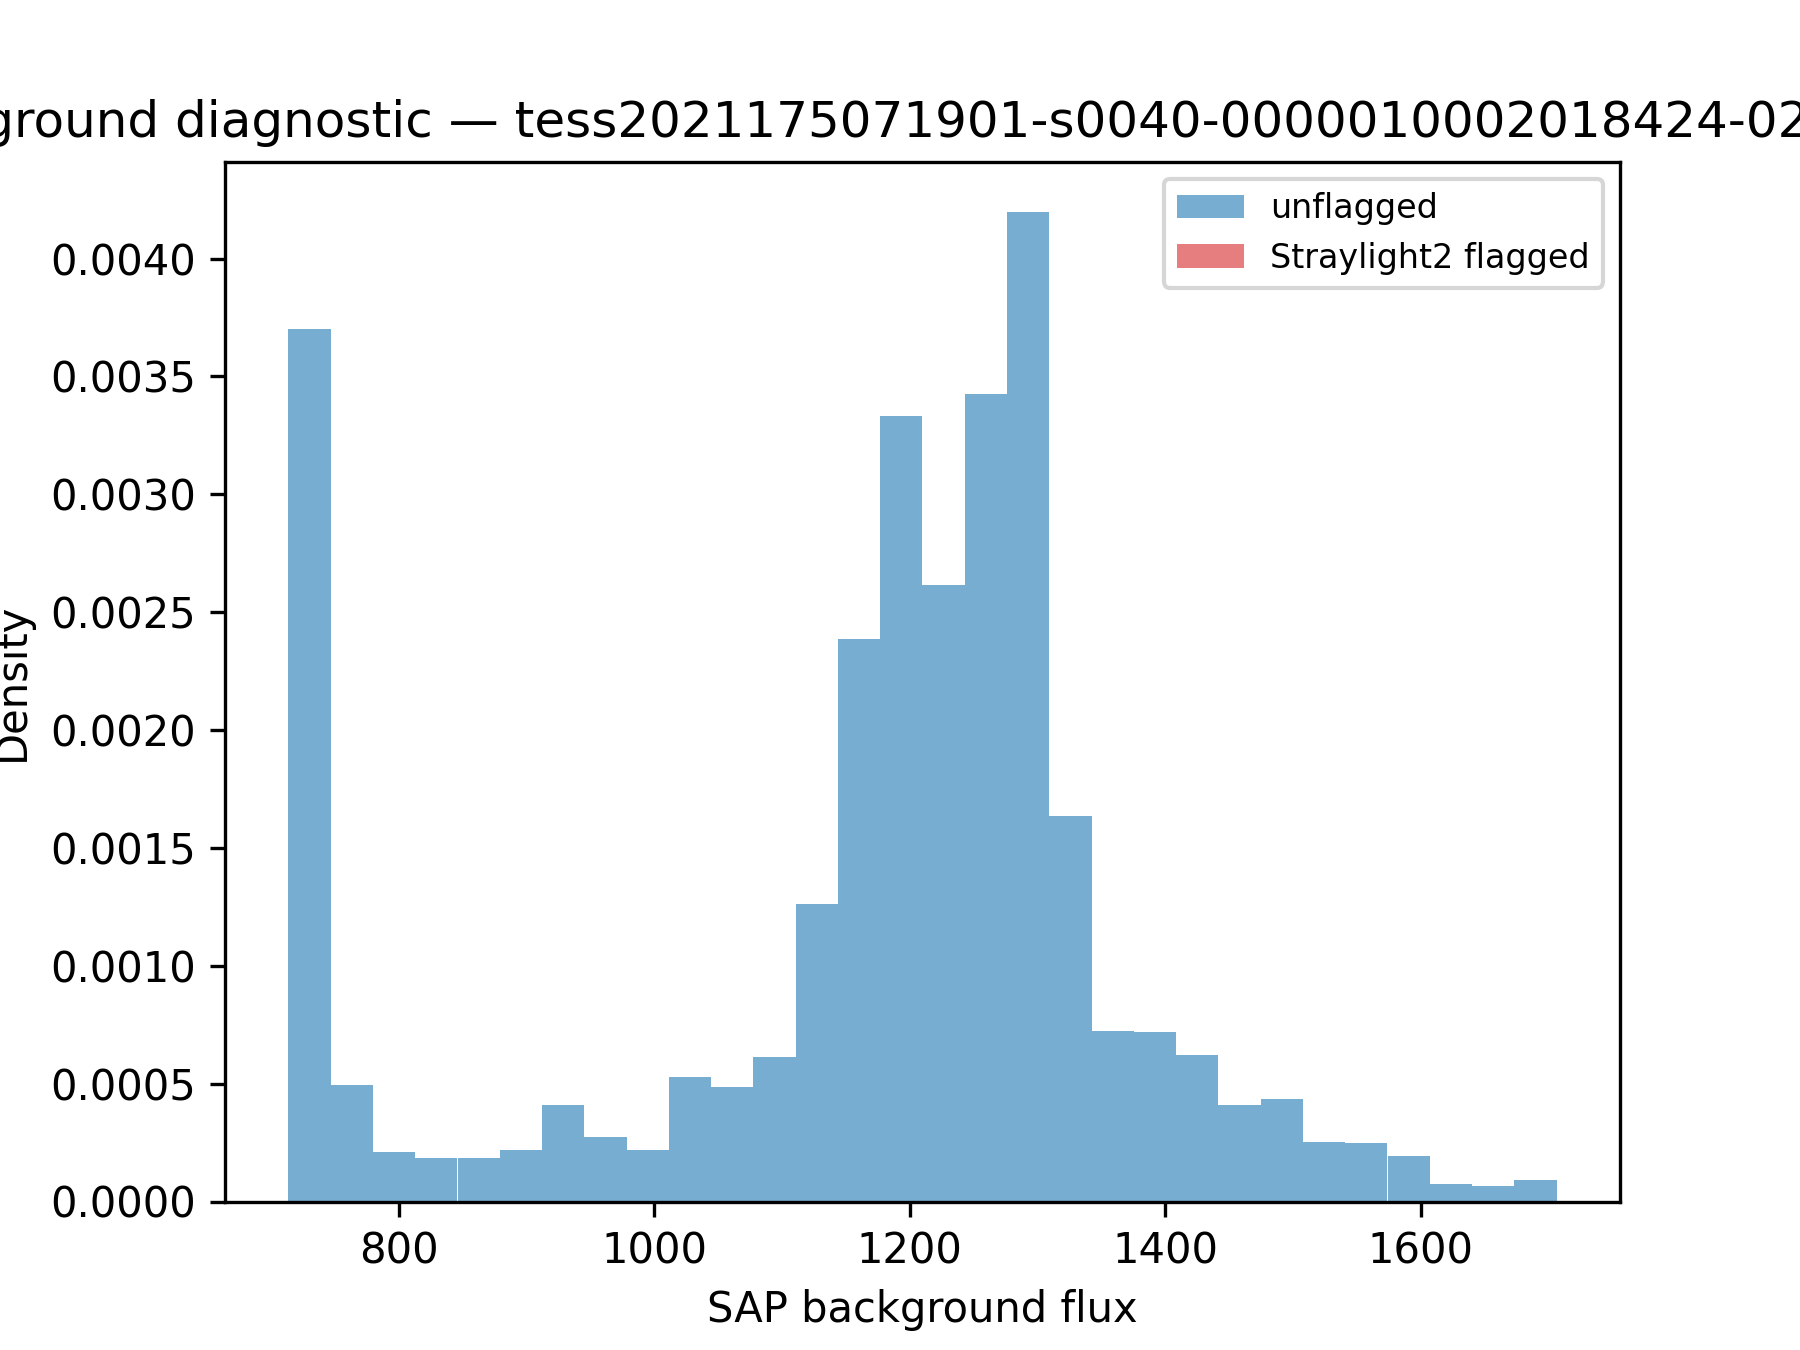
\includegraphics[width=0.6\textwidth]{../figures/fig05_background_diagnostic.png}
  \caption{Real SAP background flux distribution, one target; the
  Straylight2-flagged histogram is empty (zero flagged cadences,
  Section~\ref{sec:results}).}
  \label{fig:background}
\end{figure}

\bibliographystyle{plain}
\bibliography{references}
\end{document}
